\newpage
\subsection{Anexo}
\begin{figure}[H]
    \centering
	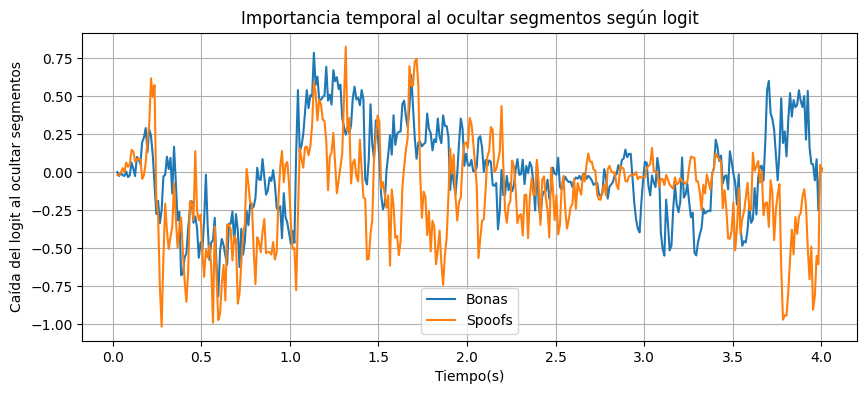
\includegraphics[width=\textwidth]{imagenes/AASIST_global_occlusion_temp_logit.png}
	\caption{Resultados de ``logit'' de la ocultación temporal en AASIST.}
    \label{fig:AASIST_global_occlusion_temporal_logit}
\end{figure}

\begin{figure}[H]
    \centering
	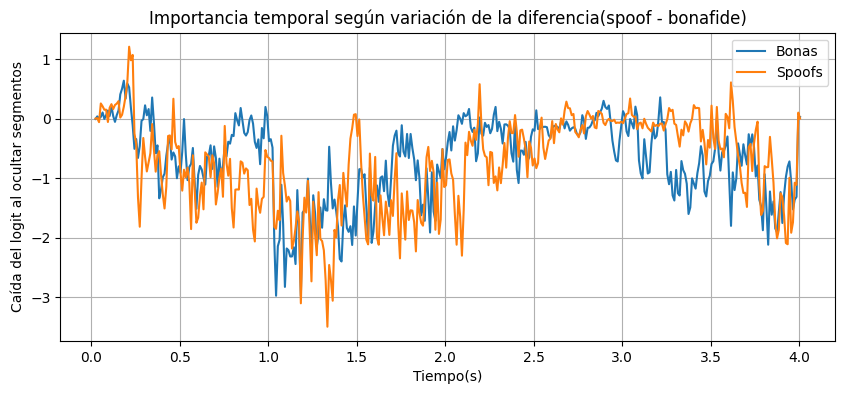
\includegraphics[width=\textwidth]{imagenes/AASIST_global_occlusion_temp_margin.png}
	\caption{Resultados de margen de la ocultación temporal en AASIST.}
    \label{fig:AASIST_global_occlusion_temporal_margin}
\end{figure}

\begin{figure}[H]
    \centering
	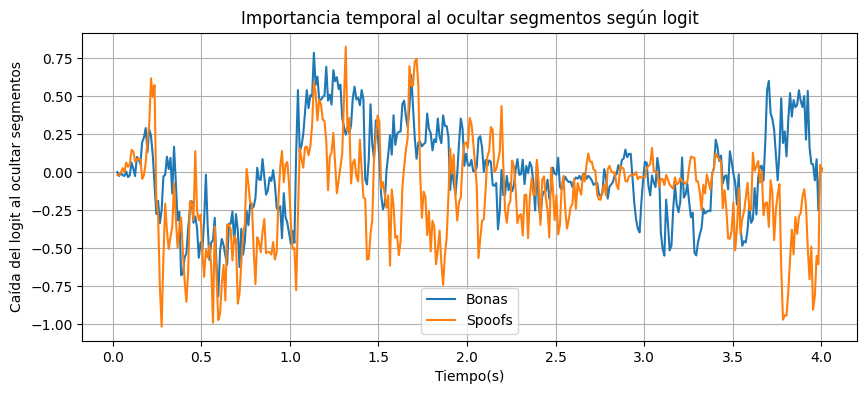
\includegraphics[width=\textwidth]{imagenes/AASIST_global_occlusion_frec_logit.png}
	\caption{Resultados de ``logit'' de la ocultación frecuencial en AASIST.}
    \label{fig:AASIST_global_occlusion_frecuencial_logit}
\end{figure}

\begin{figure}[H]
    \centering
	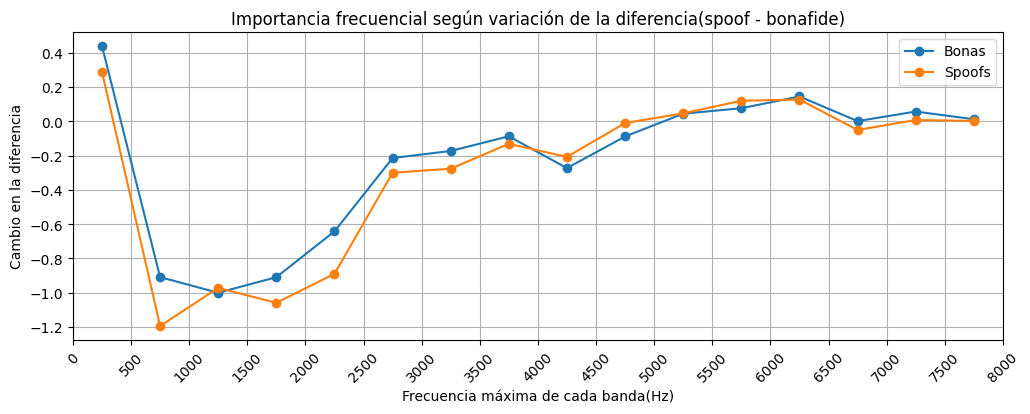
\includegraphics[width=\textwidth]{imagenes/AASIST_global_occlusion_frec_margin.png}
	\caption{Resultados de margen de la ocultación frecuencial en AASIST.}
    \label{fig:AASIST_global_occlusion_frecuencial_margin}
\end{figure}

\begin{figure}[H]
    \centering
    \begin{subfigure}[t]{0.49\textwidth}
        \centering
        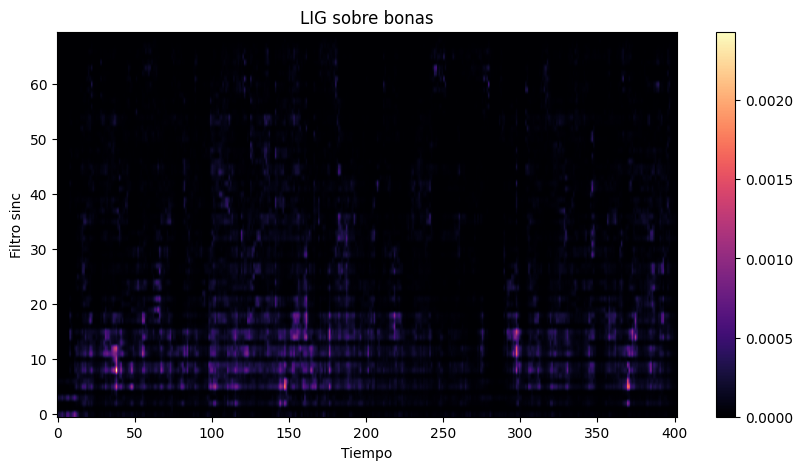
\includegraphics[width=\linewidth]{imagenes/AASIST_global_LIG_bonas.png}
        \caption{Mapa filtro-tiempo generado con IG para ``bonas''.}
        \end{subfigure}
    \hfill
    \begin{subfigure}[t]{0.49\textwidth}
        \centering
        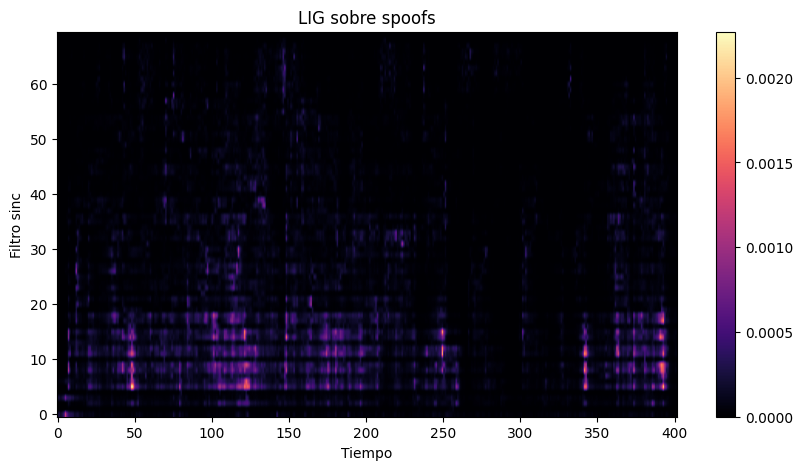
\includegraphics[width=\linewidth]{imagenes/AASIST_global_LIG_spoofs.png}
        \caption{Mapa filtro-tiempo generado con IG para ``spoofs''.}
    \end{subfigure}
    \caption{Mapas filtro-tiempo de la capa sinc-convolution generados con IG.}
    \label{fig:AASIST_global_LIG_mapas}
\end{figure}

\begin{figure}[H]
    \centering
    \begin{subfigure}[t]{0.49\textwidth}
        \centering
        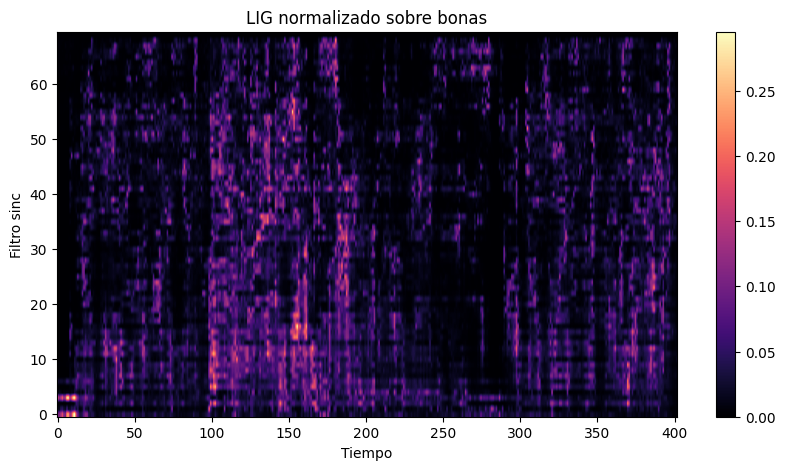
\includegraphics[width=\linewidth]{imagenes/AASIST_global_LIG_bonas_norm.png}
        \caption{Mapa filtro-tiempo normalizado generado con IG para ``bonas''.}
        \end{subfigure}
    \hfill
    \begin{subfigure}[t]{0.49\textwidth}
        \centering
        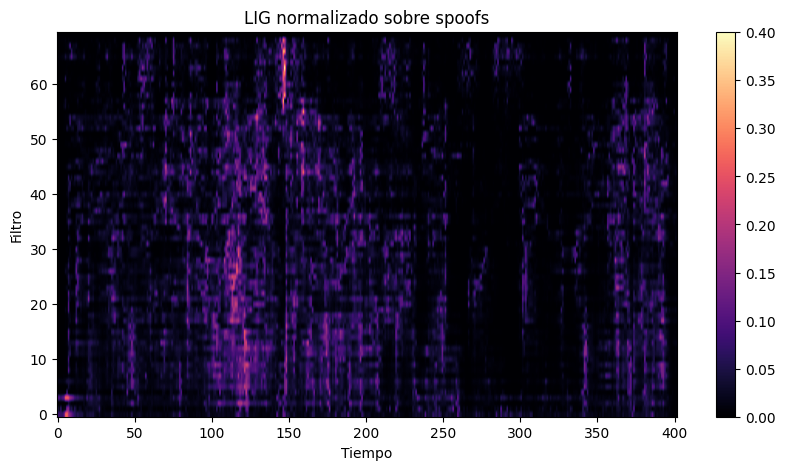
\includegraphics[width=\linewidth]{imagenes/AASIST_global_LIG_spoofs_norm.png}
        \caption{Mapa filtro-tiempo normalizado generado con IG para ``spoofs''.}
    \end{subfigure}
    \caption{Mapas filtro-tiempo de la capa sinc-convolution generados con IG normalizados.}
    \label{fig:AASIST_global_LIG_mapas_norm}
\end{figure}

\begin{figure}[H]
    \centering
	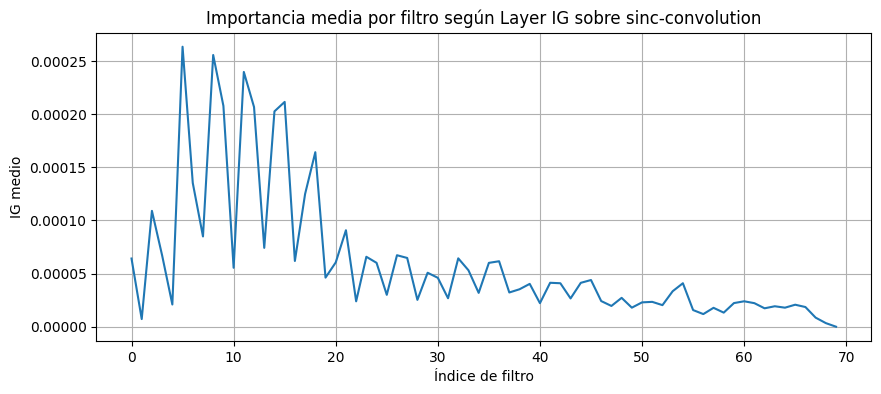
\includegraphics[width=\textwidth]{imagenes/AASIST_global_LIG_grafica.png}
	\caption{Gráfica filtro-tiempo de la capa sinc-convolution.}
    \label{fig:AASIST_global_LIG_grafica}
\end{figure}

\begin{figure}[H]
    \centering
	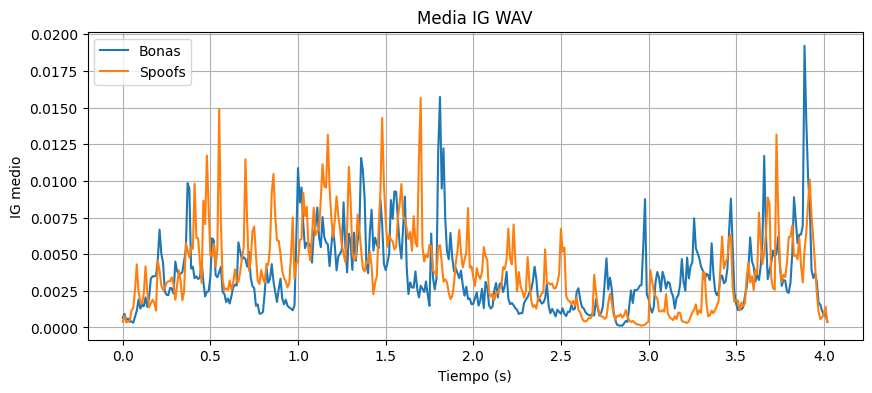
\includegraphics[width=\textwidth]{imagenes/AASIST_global_IG_audio.png}
	\caption{Importancia temporal al aplicar IG sobre onda de audio cruda.}
    \label{fig:AASIST_global_IG_audio}
\end{figure}

\begin{figure}[H]
    \centering
    \begin{subfigure}[t]{0.49\textwidth}
        \centering
        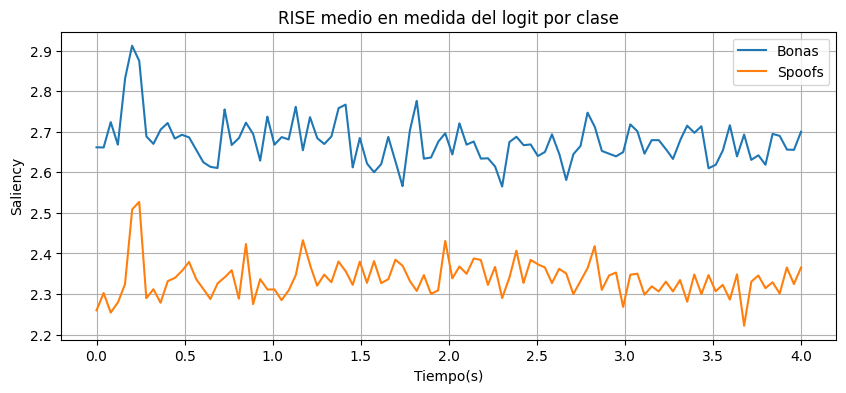
\includegraphics[width=\linewidth]{imagenes/AASIST_global_RISE_logit.png}
         \caption{Resultados de ``logit'' usando RISE.}
        \end{subfigure}
    \hfill
    \begin{subfigure}[t]{0.49\textwidth}
        \centering
        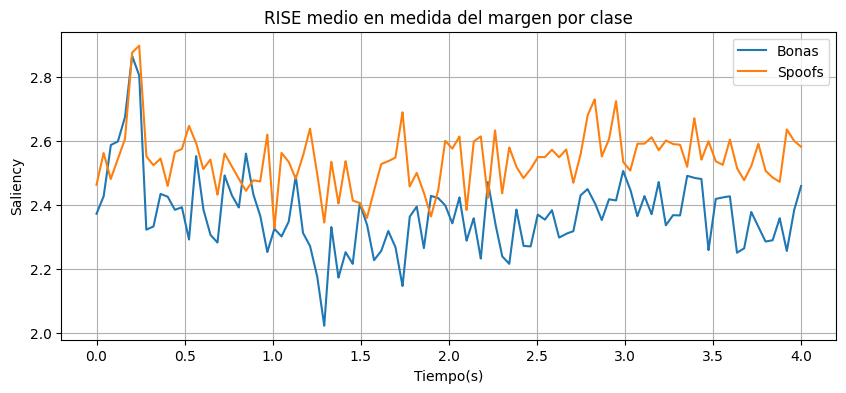
\includegraphics[width=\linewidth]{imagenes/AASIST_global_RISE_margen.png}
        \caption{Resultados de ``margin'' usando RISE.}
    \end{subfigure}
    \caption{Resultados de RISE.}
    \label{fig:AASIST_global_RISE}
\end{figure}

\begin{figure}[H]
    \centering
    \begin{subfigure}[t]{0.49\textwidth}
        \centering
        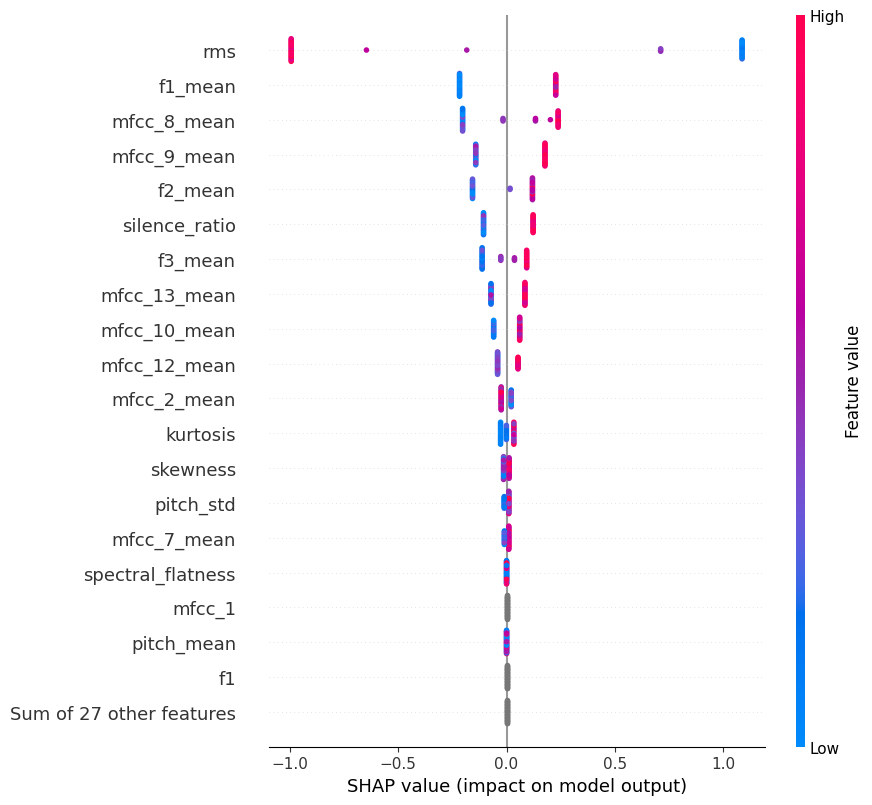
\includegraphics[width=\linewidth]{imagenes/AASIST_global_SHAP_clas.png}
        \caption{Agrupación de las gráficas SHAP del clasificador.}
        \end{subfigure}
    \hfill
    \begin{subfigure}[t]{0.49\textwidth}
        \centering
        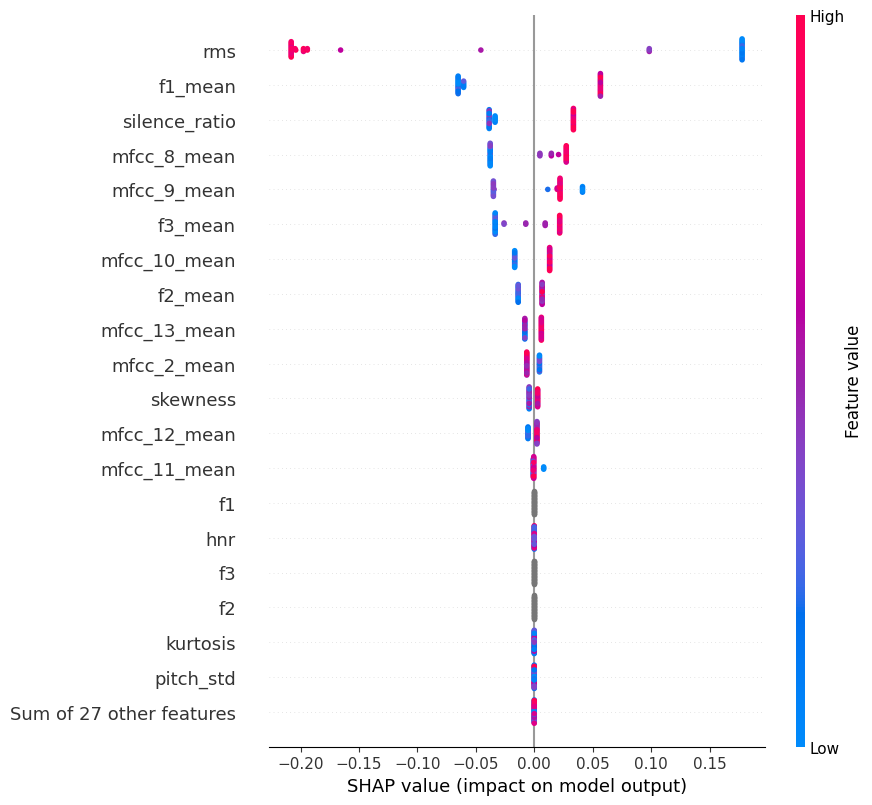
\includegraphics[width=\linewidth]{imagenes/AASIST_global_SHAP_reg.png}
        \caption{Agrupación de las gráficas SHAP del regresor.}
    \end{subfigure}
    \caption{Gráficas de importancia global de SHAP para el clasificador y el regresor.}
    \label{fig:AASIST_global_SHAP}
\end{figure}





